\documentclass[review,12pt,authoryear]{elsarticle}

\usepackage{amsmath,amssymb,amsfonts,amsthm}
\usepackage{booktabs}
\usepackage{graphicx}
\usepackage{hyperref}
\usepackage{setspace}
\usepackage{caption}
\usepackage{subcaption}
\usepackage{microtype}
\usepackage{tabularx}
\usepackage{enumitem}
\usepackage{geometry}
\geometry{margin=1in}

\hypersetup{
    colorlinks=true,
    linkcolor=blue,
    citecolor=blue,
    urlcolor=blue
}

\journal{International Review of Financial Analysis}

\begin{document}

\begin{frontmatter}

\title{Causal Emergence in U.S. Equity Industry Portfolios: Dynamic Organization and Effective Dimensionality During Systemic Stress}

\author{}

\begin{abstract}
This paper investigates whether cross-sector equity returns exhibit causal emergence, such that a macroscopic coarse-graining of industry portfolios contains higher effective transition information per degree of freedom than its constituent microscopic assets. Applying continuous-state information theory to daily U.S. equity industry portfolio returns from January 1990 to June 2026, we formulate the Causal Emergence Financial Index ($\mathrm{CEFI}_t$, measured in $\mathrm{nats/DOF}$) and estimate the Causal Effective Dimension ($q_t^*$) via Riemannian optimization on Stiefel manifolds under scale-adaptive Gaussian interventions. Benchmarking against a four-tier hierarchy of matched surrogate null models ($B=9,999$ for primary nulls), we evaluate historical dynamics across calm and stress regimes. After Holm-Bonferroni adjustment across the primary hypothesis family, no individual comparison rejects at the 5\% family-wise error rate ($p_{\text{Holm}} \ge 0.1092$). While observed emergence is statistically consistent with surrogate persistence in the 2005 calm benchmark ($p_{\text{Holm}} \ge 0.3480$), during the March 2020 COVID shock observed emergence shows nominal elevation relative to static correlation modes ($p_{\text{emp}} = 0.0182, z = +2.40$), but remains consistent with cross-lag network isolation ($p_{\text{emp}} = 0.2893, p_{\text{Holm}} = 0.4118$). Under the baseline Gaussian intervention scale ($\kappa = 1.0$), 98.94\% of historical rolling windows select low causal effective dimensions ($q^* \le 4$, with modal $q^* = 1$ accounting for 63.8\% of all windows and 87.7\% satisfying $q^* \le 2$). Because matched surrogate models without cross-lag structure also select modal $q_0^* = 1$, low-dimensional selection reflects the per-degree-of-freedom optimization criterion rather than autonomous proof of emergent market organization. Across 870 historical rolling windows, $\mathrm{CEFI}_t$ exhibits positive concordance with the analytical Gaussian SVD emergence benchmark (Pearson $\rho = 0.819$, Spearman $\rho_S = 0.821$, with 87.7\% dimensional agreement within $\pm 1$ dimension and 63.2\% exact match). These findings indicate that continuous causal emergence provides a descriptive information-theoretic measure of collective market organization and transition concentration during systemic stress.
\end{abstract}

\begin{keyword}
Causal Emergence \sep Market Organization \sep Systemic Stress \sep Effective Information \sep Stiefel Manifold \sep Effective Dimensionality
\end{keyword}

\end{frontmatter}

\doublespacing

\section{Introduction}
\label{sec:intro}

The transmission of distress across equity markets has traditionally been studied through the lens of contemporaneous co-movement, cross-sectional factor exposure, and pairwise connectedness \citep{billio2012econometric, diebold2012better, adrian2016covar, brownlees2017srisk}. During periods of severe market instability, asset returns frequently exhibit heightened cross-sectional correlation and variance concentration, phenomena commonly described as financial contagion or systemic fragility \citep{acharya2017measuring, kritzman2011principal}. However, standard econometrics evaluates financial dynamics predominantly at the observed microscopic asset resolution or through unconditional factor projections. It does not address a distinct architectural question: \emph{does a distressed financial network develop macroscopic dynamical organization, such that a coarse-grained representation of the network possesses greater effective transition information per degree of freedom than its underlying constituent assets?}

The financial relevance of this question lies in distinguishing between two distinct empirical features: (i) common simultaneous market stress, where asset returns experience contemporaneous shocks driven by common factors without structured lead-lag transmission; and (ii) organized lagged propagation across sectors, where past industry performance informs one-step ahead conditional transitions. While static covariance metrics and absorption ratios capture contemporaneous variance concentration, they cannot determine whether intertemporal transitions concentrate on a low-dimensional manifold that enhances dynamical predictability relative to noisy microscopic returns.

In the physics of complex systems and information theory, the formal framework of \emph{Causal Emergence} (CE), introduced by \citet{hoel2013quantifying} and extended by \citet{klein2020emergence} and \citet{rosas2020reconciling}, demonstrates that macroscopic representations of noisy or degenerate networks can exhibit higher \emph{Effective Information} ($EI$) than their microscopic descriptions. By grouping or projecting micro-level states onto an optimal lower-dimensional subspace, macro coarse-graining can average out idiosyncratic noise while concentrating intertemporal transition dynamics. Recent mathematical advances have derived exact analytical formulations of causal emergence for continuous-state linear stochastic iterative systems \citep{liu2024exact, liu2025singular, yang2025finding}.

This paper develops a rolling empirical implementation of continuous-state causal emergence using daily U.S. industry portfolio returns from January 1990 to June 2026. We model the cross-section of industry portfolio returns through continuous-state linear Gaussian Vector Autoregressive transition models (VAR(1)). Using Riemannian gradient ascent on Stiefel manifolds, we optimize an orthogonal projection matrix $\mathbf{W} \in \mathcal{V}_q(\mathbb{R}^p)$ that maximizes macro effective information across all potential dimensions $q \in \{1, \dots, p-1\}$. We define two central statistics:
\begin{enumerate}[label=(\roman*)]
    \item The \emph{Causal Emergence Financial Index} ($\mathrm{CEFI}_t$), measuring the maximal causal information rate per degree of freedom gained through macroscopic coarse-graining (expressed in nats per degree of freedom, $\mathrm{nats/DOF}$):
    \begin{equation}
    \mathrm{CEFI}_t = \max_{1 \le q < p} \left[ \frac{EI_{q,t}^*}{q} - \frac{EI_{p,t}}{p} \right]
    \end{equation}
    \item The \emph{Causal Effective Dimension} ($q_t^*$), identifying the optimizer-selected macro dimension at which causal transition concentration is maximized:
    \begin{equation}
    q_t^* = \arg\max_{1 \le q < p} \left[ \frac{EI_{q,t}^*}{q} - \frac{EI_{p,t}}{p} \right]
    \end{equation}
\end{enumerate}

To ensure that the measure is invariant to common scalar changes in return units (e.g., decimal vs. percentage returns), we introduce an isotropic Gaussian intervention scaled by average channel energy, combined with an energy-scaled ridge regularizer. Because positive $\mathrm{CEFI}_t$ can arise mechanically under finite-sample optimization, we evaluate historical estimates against a four-tier hierarchy of matched surrogate null models ($B=9,999$ for primary nulls and $B=999$ for auxiliary nulls), including a cross-lag network isolation null ($H_0^{\text{diag+contemp}}$) that preserves own-lag persistence and the full empirical contemporaneous innovation covariance matrix $\boldsymbol{\Sigma}_\varepsilon$.

The empirical analysis delivers several main descriptive findings:
\begin{enumerate}
    \item \textbf{Descriptive Variation Across Historical Stress Episodes:} Positive causal emergence is observed across both calm and crisis regimes, while its magnitude and descriptive separation from matched surrogate nulls vary across market states. In the 2005 calm-market benchmark window, observed emergence ($\mathrm{CEFI}_{\text{obs}} = 0.2023\ \mathrm{nats/DOF}, q^* = 1$) is statistically consistent with surrogate persistence ($H_0^{\text{static}} p_{\text{Holm}} = 0.3480$; $H_0^{\text{diag+contemp}} p_{\text{Holm}} = 0.4118$). At the GFC and COVID benchmark windows, observed emergence exceeds the 2005 calm-benchmark value: during the 2008 GFC peak ($\mathrm{CEFI}_{\text{obs}} = 0.3656\ \mathrm{nats/DOF}, q^* = 1$), emergence approaches the surrogate boundary ($p_{\text{emp}} = 0.0572, p_{\text{Holm}} = 0.2860$), while during the March 2020 COVID shock ($\mathrm{CEFI}_{\text{obs}} = 0.3342\ \mathrm{nats/DOF}, q^* = 2$), observed emergence nominally exceeds static correlation modes ($p_{\text{emp}} = 0.0182, z = +2.40, p_{\text{Holm}} = 0.1092$). Crucially, after Holm-Bonferroni adjustment across the primary hypothesis family, no primary test rejects at the 5\% family-wise significance level.
    \item \textbf{Descriptive Separation from Cross-Lag Isolation:} The descriptive excess of observed emergence over the cross-lag network isolation null ($\mathrm{CEFI}_{\text{obs}} - \mathbb{E}[\mathrm{CEFI}_0^{\text{diag+contemp}}]$) is larger at the GFC peak (+0.0778 nats/DOF) than at the calm benchmark (+0.0370 nats/DOF). However, this difference represents descriptive historical variation, as the corresponding primary null comparison does not reject after multiplicity adjustment ($p_{\text{Holm}} = 0.2860$), and during COVID observed emergence remains fully consistent with cross-lag isolation ($p_{\text{emp}} = 0.2893$).
    \item \textbf{Persistent Low Dimensionality Under Baseline Interventions:} Across the complete 1992--2026 sample, 98.94\% of historical rolling windows select low causal effective dimensions ($q^* \le 4$, with modal $q^* = 1$ accounting for 63.8\% of all windows and 87.7\% satisfying $q^* \le 2$). Importantly, matched surrogate null models also overwhelmingly select modal $q_0^* = 1$, demonstrating that low-dimensional concentration reflects the per-degree-of-freedom optimization criterion rather than autonomous proof of non-null emergent market organization. Furthermore, this dimensional selection is conditional on the baseline Gaussian intervention scale ($\kappa = 1.0$), with smaller intervention scales shifting modal dimension toward the microscopic boundary.
    \item \textbf{Cross-Method Concordance:} Across 870 historical rolling windows, $\mathrm{CEFI}_t$ exhibits positive concordance with the analytical Gaussian SVD emergence benchmark of \citet{liu2025singular} (Pearson $\rho = 0.819$, Spearman $\rho_S = 0.821$, with 87.7\% dimensional agreement within $\pm 1$ dimension and 63.2\% exact match), supporting cross-method theoretical concordance under Gaussian assumptions, while exhibiting substantially lower concordance with the bounded-uniform intervention framework ($\rho = 0.445, \rho_S = 0.356$).
    \item \textbf{Cross-Partition and Industry-Granularity Sensitivity (FF49 Replication):} Applying the framework across the 49 Fama-French industry portfolios cross-section ($p=49$) confirms persistent low-dimensional selection under finer industrial granularity (mean $\mathrm{CEFI} = 0.3592\ \mathrm{nats/DOF}$, modal $q^* = 1$, 97.13\% satisfying $q^* \le 4$).
\end{enumerate}

The remainder of the paper is organized as follows. Section \ref{sec:literature} reviews the related literature. Section \ref{sec:methodology} presents the mathematical methodology and Stiefel optimization. Section \ref{sec:data} describes the data and matched null hierarchy. Section \ref{sec:results} reports empirical findings. Section \ref{sec:robustness} provides theoretical benchmarking and robustness checks. Section \ref{sec:discussion} discusses economic interpretations. Section \ref{sec:limitations} outlines limitations, and Section \ref{sec:conclusion} concludes.

\section{Related Literature and Conceptual Foundations}
\label{sec:literature}

\subsection{Systemic Risk and Financial Connectedness}
Our work relates to the econometric literature on systemic financial risk, market connectedness, and cross-sectoral spillover networks \citep{billio2012econometric, diebold2012better, diebold2014network, adrian2016covar, brownlees2017srisk}. Seminal contributions have demonstrated the power of high-dimensional rolling connectedness and frequency-dependent spillovers for tracking systemic fragility \citep{demirer2018estimating, barunik2018measuring}. Recent contributions in the \emph{International Review of Financial Analysis} and related finance literature have highlighted the importance of dynamic connectedness, transfer entropy, partial Granger networks, and multilayer risk transmission during crisis episodes \citep{ahelegbey2022network, yousaf2022linkages, mensi2021spillovers, bouri2021return, yang2023modeling, ardakani2024transfer, yao2025interindustry}. 

While these frameworks effectively quantify contemporaneous co-movement, tail dependence, or pairwise linear spillovers at the observed microscopic resolution, they do not examine whether a macroscopic aggregation of the system can exhibit higher deterministic causal transition structure than the underlying portfolio components.

\subsection{Information Theory, Entropy, and Dimensionality in Finance}
Information-theoretic concepts have a rich history in quantitative finance. Non-parametric measures such as Shannon entropy, transfer entropy, and mutual information have been applied to detect non-linear information flows and cross-market spillover networks \citep{schreiber2000measuring, dimpfl2013using, bekiros2017information}. Spectral measures of effective dimensionality, such as the effective rank of a covariance matrix \citep{roy2007effective}, have been employed to quantify market concentration during crises.

However, existing spectral dimensionality metrics depend exclusively on the static contemporaneous covariance matrix $\boldsymbol{\Sigma}_x$. They do not incorporate intertemporal transition dynamics ($\mathbf{A}$) or innovation noise covariance ($\boldsymbol{\Sigma}_\varepsilon$). In contrast, the Causal Effective Dimension ($q_t^*$) developed in this paper incorporates transition mechanics and innovation uncertainty simultaneously under an interventional perturbation framework.

\subsection{Causal Emergence in Complex Dynamical Systems}
The theory of causal emergence originated in discrete Markov chains to formalize how coarse-grained macroscopic states can reduce degeneracy and noise \citep{hoel2013quantifying, hoel2017when, klein2020emergence}. \citet{rosas2020reconciling} unified causal emergence with partial information decomposition, distinguishing between downward causation and synergistic emergence.

Recent mathematical physics research has extended causal emergence to continuous-state stochastic dynamical systems. \citet{liu2024exact} derived exact continuous effective information and emergence conditions for linear stochastic systems under uniform bounded interventions. \citet{liu2025singular} developed an analytical singular value decomposition (SVD) perspective for Gaussian iterative dynamics, demonstrating equivalence conditions between SVD-based and EI-based emergence. \citet{yang2025finding} formulated machine learning architectures to discover emergence from observational data. Our paper adapts these continuous-state foundations to empirical financial econometrics, rolling-window market monitoring, and matched-null inference.

\section{Mathematical Methodology}
\label{sec:methodology}

\subsection{Reduced-Form Linear Continuous-State Markov Dynamics}
Let $\mathbf{x}_t = (x_{1,t}, x_{2,t}, \dots, x_{p,t})^\top \in \mathbb{R}^p$ denote a $p$-dimensional column vector of daily portfolio returns. We model the transition dynamics via a continuous-state first-order Vector Autoregression, $\text{VAR}(1)$:
\begin{equation}
\mathbf{x}_{t+1} = \mathbf{A}\mathbf{x}_t + \boldsymbol{\varepsilon}_{t+1}, \qquad \boldsymbol{\varepsilon}_{t+1} \sim \mathcal{N}(\mathbf{0}, \boldsymbol{\Sigma}_\varepsilon)
\label{eq:var1_model}
\end{equation}
where $\mathbf{A} \in \mathbb{R}^{p \times p}$ is the transition matrix, and $\boldsymbol{\varepsilon}_{t+1}$ is a vector of Gaussian innovations with positive-definite covariance matrix $\boldsymbol{\Sigma}_\varepsilon \in \mathbb{R}^{p \times p}$. 

Let $\mathbf{X}_{\text{lag}} \in \mathbb{R}^{(T-1) \times p}$ and $\mathbf{X}_{\text{lead}} \in \mathbb{R}^{(T-1) \times p}$ denote the data matrices whose $t$-th rows contain $\mathbf{x}_t^\top$ and $\mathbf{x}_{t+1}^\top$, respectively. In row-regression format, $\mathbf{X}_{\text{lead}} \approx \mathbf{X}_{\text{lag}}\mathbf{A}^\top$. To guarantee scale invariance and prevent overfitting in finite rolling estimation windows, $\mathbf{A}$ is estimated via trace-scaled ridge regression:
\begin{equation}
\hat{\mathbf{A}} = \mathbf{X}_{\text{lead}}^\top \mathbf{X}_{\text{lag}} \left( \mathbf{X}_{\text{lag}}^\top \mathbf{X}_{\text{lag}} + \lambda_t \mathbf{I}_p \right)^{-1}, \qquad \lambda_t = \lambda_0 \cdot \frac{\operatorname{Tr}(\mathbf{X}_{\text{lag}}^\top \mathbf{X}_{\text{lag}})}{p}
\label{eq:scaled_ridge}
\end{equation}
with baseline regularization parameter $\lambda_0 = 10^{-4}$. Scaling the ridge penalty proportionally to the empirical trace of the Gram matrix ensures that $\hat{\mathbf{A}}$ is strictly invariant under common scalar rescalings of return units ($\mathbf{X} \to c\mathbf{X}$). The residual covariance matrix $\boldsymbol{\Sigma}_\varepsilon$ is estimated using Ledoit-Wolf analytical shrinkage \citep{ledoit2004well}, which preserves scale equivariance ($\boldsymbol{\Sigma}_\varepsilon \to c^2 \boldsymbol{\Sigma}_\varepsilon$) and guarantees strict positive definiteness ($\lambda_{\min}(\boldsymbol{\Sigma}_\varepsilon) > 0$). The unconditional covariance matrix of the state vector is denoted by $\boldsymbol{\Sigma}_x = \operatorname{Cov}(\mathbf{x}_t)$.

\paragraph{Delimitation of Causal Terminology}
The term \emph{causal} is used throughout this paper strictly in the intervention-based information-theoretic sense of Effective Information conditional on the estimated stochastic transition operator \citep{hoel2013quantifying, liu2024exact}. It should not be interpreted as structural economic causality in the sense of Structural VAR (SVAR) identification, instrumental variables, potential outcomes, or Pearlian structural causal DAGs. The estimated VAR transition matrix $\mathbf{A}$ provides a reduced-form dynamical representation of market co-movements upon which counterfactual isotropic Gaussian intervention distributions are evaluated.

\subsection{Isotropic Scale-Invariant Gaussian Interventions and Effective Information}
Effective Information ($EI$) quantifies the mutual information between an intervened state $do(\mathbf{x}_t)$ and the subsequent state $\mathbf{x}_{t+1}$ \citep{hoel2013quantifying}:
\begin{equation}
EI(\mathbf{x}) = I(do(\mathbf{x}_t); \mathbf{x}_{t+1}) = H(\mathbf{x}_{t+1} \mid do) - H(\mathbf{x}_{t+1} \mid \mathbf{x}_t)
\label{eq:ei_def_eq}
\end{equation}
Under Gaussian transition dynamics, the conditional entropy is given by $H(\mathbf{x}_{t+1} \mid \mathbf{x}_t) = \frac{p}{2}\ln(2\pi e) + \frac{1}{2}\ln\det(\boldsymbol{\Sigma}_\varepsilon)$.

To evaluate interventional causality independently of observational factor orientations, we apply an isotropic Gaussian intervention $do(\mathbf{x}_t) \sim \mathcal{N}(\mathbf{0}, \sigma_{do,t}^2 \mathbf{I}_p)$. Conditional on a fixed isotropic covariance, the Gaussian distribution maximizes differential entropy. To ensure that $EI$ is strictly invariant to common scalar changes in return units, we set the intervention variance proportionally to the average observed state variance:
\begin{equation}
\sigma_{do,t}^2 = \kappa^2 \cdot \frac{\operatorname{Tr}(\boldsymbol{\Sigma}_{x,t})}{p}
\label{eq:scale_inv_def}
\end{equation}
where $\kappa > 0$ is a dimensionless scale parameter ($\kappa = 1.0$ by default). Under this intervention, $\mathbf{x}_{t+1} \mid do \sim \mathcal{N}(\mathbf{0}, \sigma_{do,t}^2 \mathbf{A}\mathbf{A}^\top + \boldsymbol{\Sigma}_\varepsilon)$. In whitened coordinates, the transition covariance is evaluated via the symmetric positive definite (SPD) matrix:
\begin{equation}
\mathbf{M}_{\text{micro}} = \mathbf{I}_p + \sigma_{do,t}^2 \boldsymbol{\Sigma}_\varepsilon^{-1/2} \mathbf{A}\mathbf{A}^\top \boldsymbol{\Sigma}_\varepsilon^{-1/2}
\label{eq:m_micro_spd}
\end{equation}
By Sylvester's determinant identity ($\det(\mathbf{I} + \mathbf{A}\mathbf{B}) = \det(\mathbf{I} + \mathbf{B}\mathbf{A})$), this possesses the identical positive determinant to the non-symmetric matrix $\mathbf{I}_p + \sigma_{do,t}^2 \mathbf{A}\mathbf{A}^\top \boldsymbol{\Sigma}_\varepsilon^{-1}$. The closed-form continuous Effective Information is therefore:
\begin{equation}
EI_{\text{micro}}(\mathbf{x}) = \frac{1}{2} \ln \det\left( \mathbf{M}_{\text{micro}} \right) = \frac{1}{2} \ln \det\left( \mathbf{I}_p + \sigma_{do,t}^2 \mathbf{A}\mathbf{A}^\top \boldsymbol{\Sigma}_\varepsilon^{-1} \right)
\label{eq:ei_micro_closed}
\end{equation}
where numerical evaluation is executed stably on the whitened SPD form via Cholesky decomposition ($\boldsymbol{\Sigma}_\varepsilon = \mathbf{L}\mathbf{L}^\top$, $\mathbf{Y} = \mathbf{L}^{-1}\mathbf{A}$, $\mathbf{M}_{\text{micro}} = \mathbf{I}_p + \sigma_{do,t}^2 \mathbf{Y}\mathbf{Y}^\top$).

\subsection{Macro Coarse-Graining and Stiefel Manifold Optimization}
We define a linear coarse-graining mapping from the $p$-dimensional micro-system to a $q$-dimensional macro-system ($q < p$) via an orthogonal projection matrix $\mathbf{W} \in \mathbb{R}^{q \times p}$:
\begin{equation}
\mathbf{y}_t = \mathbf{W}\mathbf{x}_t, \qquad \mathbf{W}\mathbf{W}^\top = \mathbf{I}_q
\end{equation}
The matrix $\mathbf{W}$ resides on the row-Stiefel manifold $\mathcal{V}_q(\mathbb{R}^p) = \{ \mathbf{W} \in \mathbb{R}^{q \times p} : \mathbf{W}\mathbf{W}^\top = \mathbf{I}_q \}$. 

\paragraph{Interventional Macro Channel Construction}
Following \citet{liu2024exact}, an intervention on the macro-state $do(\mathbf{y}_t)$ is lifted to the micro-state via the canonical right inverse $do(\mathbf{x}_t) = \mathbf{W}^\top do(\mathbf{y}_t)$. Projecting the resulting transition back via $\mathbf{W}$ defines the constructed macro interventional channel:
\begin{equation}
\mathbf{y}_{t+1} = \mathbf{A}_M \mathbf{y}_t + \boldsymbol{\varepsilon}_{M, t+1}, \qquad \mathbf{A}_M = \mathbf{W}\mathbf{A}\mathbf{W}^\top, \quad \boldsymbol{\Sigma}_M = \mathbf{W}\boldsymbol{\Sigma}_\varepsilon \mathbf{W}^\top
\label{eq:macro_dynamics_def}
\end{equation}
Defining the whitened macro transition matrix:
\begin{equation}
\mathbf{M}_M(\mathbf{W}) = \mathbf{I}_q + \sigma_{do,t}^2 \boldsymbol{\Sigma}_M^{-1/2} \mathbf{A}_M \mathbf{A}_M^\top \boldsymbol{\Sigma}_M^{-1/2}
\label{eq:m_macro_spd}
\end{equation}
which is symmetric positive definite (SPD), the macro Effective Information is:
\begin{equation}
EI_q(\mathbf{W}) = \frac{1}{2} \ln \det\left( \mathbf{M}_M(\mathbf{W}) \right) = \frac{1}{2} \ln \det\left( \mathbf{I}_q + \sigma_{do,t}^2 \mathbf{A}_M \mathbf{A}_M^\top \boldsymbol{\Sigma}_M^{-1} \right)
\label{eq:ei_macro_closed}
\end{equation}
where the non-symmetric expression is determinant-equivalent by Sylvester's identity, and the whitened SPD form is evaluated numerically via the Cholesky factor of $\boldsymbol{\Sigma}_M$.

The optimal coarse-graining $\mathbf{W}_q^* = \arg\max_{\mathbf{W} \in \mathcal{V}_q(\mathbb{R}^p)} EI_q(\mathbf{W})$ is sought via Riemannian gradient ascent \citep{edelman1998geometry, absil2008optimization}. Under the canonical metric on $T_{\mathbf{W}}\mathcal{V}_q(\mathbb{R}^p)$, the Riemannian gradient is:
\begin{equation}
\operatorname{grad}_{\mathcal{R}} EI_q(\mathbf{W}) = \mathbf{G} - \mathbf{W}\mathbf{G}^\top \mathbf{W}
\end{equation}
where $\mathbf{G} = \nabla_{\mathbf{W}} EI_q(\mathbf{W}) \in \mathbb{R}^{q \times p}$ denotes the Euclidean gradient. The manifold update at iteration $k$ follows:
\begin{equation}
\mathbf{Z}_{k+1} = \mathbf{W}_k + \eta \operatorname{grad}_{\mathcal{R}} EI_q(\mathbf{W}_k), \qquad \mathbf{Z}_{k+1}^\top = \mathbf{Q}\mathbf{R}, \qquad \mathbf{W}_{k+1} = \mathbf{Q}^\top
\end{equation}
where $\mathbf{Q}\mathbf{R}$ denotes the QR factorization retracting the updated matrix back onto the row-Stiefel manifold, with step size $\eta = 0.05$. Based on a computational budget calibration against a 25-multistart/150-iteration higher-budget numerical benchmark (evaluated across 25 sample windows; see \ref{app:optimizer_calibration} and Supplementary Appendix, Section 4), the production estimator executes 100 Riemannian gradient iterations across 12 deterministic multistart initializations (including PCA projection and deterministic orthogonal bases) on $\mathcal{V}_q(\mathbb{R}^p)$. This configuration attains a 1.82\% median objective gap (95th percentile gap 11.70\%) relative to the higher-budget benchmark, with 92.0\% exact agreement in selected dimension and 100.0\% recovery within $\pm 1$. We emphasize that the 25/150 benchmark is itself a higher-budget numerical approximation rather than a theoretical global optimum. The identical optimization budget (12 restarts / 100 iterations) is strictly applied across both observed market windows and surrogate null realizations, eliminating differential search-budget bias between observed and surrogate test statistics.

\subsection{Causal Emergence Financial Index, Effective Dimension, and Tie-Breaking}
Because continuous $EI$ scales with state dimension, comparisons across dimensions evaluate the \emph{information rate per degree of freedom} \citep{liu2024exact}, measured in nats per degree of freedom ($\mathrm{nats/DOF}$):
\begin{equation}
\mathrm{CEFI}_t = \max_{1 \le q < p} \left[ \frac{EI_{q,t}^*}{q} - \frac{EI_{p,t}}{p} \right] \qquad [\mathrm{nats/DOF}]
\label{eq:cefi_def}
\end{equation}
\begin{equation}
q_t^* = \arg\max_{1 \le q < p} \left[ \frac{EI_{q,t}^*}{q} - \frac{EI_{p,t}}{p} \right]
\label{eq:q_star_def}
\end{equation}
Here, $q_t^*$ represents the optimizer-selected causal-effective dimension under the specified Gaussian intervention criterion. When multiple candidate dimensions $q$ achieve objective values within numerical tolerance ($\epsilon = 10^{-7}$), a deterministic tie-breaking rule selects the minimal dimension $q^* = \min \{ q : \Delta EI_q \ge \max_{k} \Delta EI_k - \epsilon \}$.

\paragraph{AI-Assisted Computational Development}
During the preparation of this work, the author used generative artificial intelligence technologies—specifically OpenAI ChatGPT (GPT-4o / o1) and Google Gemini (Gemini 1.5 Pro / Advanced)—as assistive tools for code review, algorithm optimization, and the development of numerical verification scripts. All research conceptualization, mathematical derivations, econometric specifications, empirical findings, and interpretations were directed, verified, and validated by the author, who takes full scientific responsibility for the computational methods and results in accordance with Elsevier's June 2026 AI policy.

\section{Data and Empirical Design}
\label{sec:data}

\subsection{Equity Portfolio Datasets}
Our empirical analysis uses daily value-weighted portfolio returns from the Kenneth French Data Library. The primary dataset consists of the 30 Industry Portfolios (FF30) from January 1990 to June 2026 ($T = 9,190$ trading days, $p = 30$). To evaluate industry-granularity and cross-partition sensitivity, we replicate the pipeline on the 49 Industry Portfolios (FF49, $p=49$).

\subsection{Rolling Estimation Protocol}
We employ rolling estimation windows of $W = 500$ trading days ($\sim 2$ years), stepping by 2 trading days across the 1992--2026 period ($N = 4,346$ rolling parameter estimates). At each step $t$, the trailing window $X_{t-W+1:t}$ is used to estimate $\hat{\mathbf{A}}_t$, $\boldsymbol{\Sigma}_{\varepsilon,t}$, and $\boldsymbol{\Sigma}_{x,t}$, and solve the Stiefel optimization problem for all $q \in \{1, \dots, p-1\}$. Because consecutive windows share 498 out of 500 trading days, the resulting rolling series exhibits substantial mechanical autocorrelation that persists over approximately 250 steps, which is explicitly accounted for in our inferential bandwidths using Newey-West \citep{newey1987hypothesis} covariance estimators and stationary bootstrap resampling \citep{politis1994stationary}.

\subsection{Benchmark Historical Episodes and Trailing Window Endpoints}
We evaluate four canonical historical market stress episodes:
\begin{enumerate}
    \item \textbf{2000 Dot-Com Crash}: March 1, 2000 to October 9, 2002 ($N = 327$ rolling windows; valuation bubble collapse concentrated in technology and telecom, ending at the Nasdaq bear market closing trough on October 9, 2002).
    \item \textbf{2008 Global Financial Crisis (GFC)}: October 1, 2007 to March 31, 2009 ($N = 189$ rolling windows; systemic banking contagion and credit freeze through the Q1 2009 broad market trough).
    \item \textbf{2020 COVID Shock}: February 1, 2020 to April 30, 2020 ($N = 31$ rolling windows; acute global cross-asset liquidation and lockdown shock through emergency central bank liquidity interventions).
    \item \textbf{2022 Rate Tightening}: January 1, 2022 to December 31, 2022 ($N = 125$ rolling windows; macro-monetary discount rate repricing across the full calendar year 2022 Federal Reserve rate-hiking cycle).
\end{enumerate}
Episodes (2) and (3) represent systemic liquidity and contagion crises ($N = 220$ pooled windows), whereas (1) and (4) represent broad valuation and rate repricing shocks ($N = 452$ pooled windows).

For matched-null inference, benchmark statistics are computed from 500-trading-day trailing windows ending on December 30, 2005, November 20, 2008, and March 23, 2020, corresponding respectively to the calm benchmark (calendar year-end 2005), the peak post-Lehman market liquidation week, and the global market trough of the COVID-19 pandemic selloff. Benchmark endpoints were defined prior to surrogate estimation using externally dated market stress milestones rather than post-hoc optimization of $\mathrm{CEFI}_t$.

\subsection{Hierarchy of Four Matched Surrogate Null Models}
To assess whether empirical $\mathrm{CEFI}_t$ reflects dynamic structure rather than finite-sample optimization artifacts, we evaluate four surrogate null models:
\begin{enumerate}
    \item \textbf{$H_0^{\text{circ}}$ (Circular Shift Null)}: Circularly shifts each asset column independently by random lags. Preserves marginal autocorrelation and variance, destroys cross-correlations and cross-lags.
    \item \textbf{$H_0^{\text{diag}}$ (Decoupled Diagonal VAR Null)}: Simulates an uncoupled VAR(1) with $\mathbf{D} = \operatorname{diag}(\hat{\mathbf{A}})$ and $\boldsymbol{\Sigma}_{\text{diag}} = \operatorname{diag}(\boldsymbol{\Sigma}_\varepsilon)$.
    \item \textbf{$H_0^{\text{static}}$ (Static Correlation Mode Null)}: Synchronously permutes time steps across all assets. Preserves the exact contemporaneous covariance $\boldsymbol{\Sigma}_x$, but destroys intertemporal causality $\mathbf{x}_t \to \mathbf{x}_{t+1}$.
    \item \textbf{$H_0^{\text{diag+contemp}}$ (Cross-Lag Network Isolation Null)}: Simulates $\mathbf{x}_{t+1} = \operatorname{diag}(\hat{\mathbf{A}})\mathbf{x}_t + \boldsymbol{\varepsilon}_{t+1}$ with the full empirical contemporaneous covariance $\boldsymbol{\Sigma}_\varepsilon$. Preserves univariate persistence and contemporaneous shock covariance, destroying only off-diagonal cross-lag couplings ($A_{ij} = 0, i \neq j$).
\end{enumerate}
For each regime, the observed statistic $\mathrm{CEFI}_{\text{obs}}$ is computed once with deterministic initialization and compared against $B=9,999$ surrogate replications for primary nulls ($H_0^{\text{static}}$ and $H_0^{\text{diag+contemp}}$). Empirical $p$-values are evaluated as Monte Carlo empirical tail probabilities computed with the $+1$ correction: $p_{\text{emp}} = (1 + \sum_{b=1}^B \mathbb{I}(\mathrm{CEFI}_b^{\text{null}} \ge \mathrm{CEFI}_{\text{obs}}))/(B + 1)$.

\section{Empirical Results}
\label{sec:results}

\subsection{Evidence from Matched Null Models and Mechanism Contrast}
Table \ref{tab:null_models} reports the statistical inference across calm and crisis episodes under $B=9,999$ surrogate replications for primary nulls, along with Holm-Bonferroni family-wise adjusted $p$-values ($m=6$).

\begin{table}[htbp]
\centering
\caption{Inference on Causal Emergence Across 4 Matched Null Models ($B=9,999$ for Primary Nulls, $B=999$ for Auxiliary Nulls, $q \in \{1, \dots, 29\}$)}
\label{tab:null_models}
\resizebox{\textwidth}{!}{
\begin{tabular}{llcccccccc}
\toprule
\textbf{Market Regime} & \textbf{Null Model} & $\mathbf{B}$ & $\mathbf{CEFI_{\text{obs}}}$ & $\mathbb{E}[\mathbf{CEFI_0}]$ & $\mathbf{Q_{95}}$ & $\mathbf{z_{\text{dev}}}$ & $\mathbf{p_{\text{emp}}}$ & $\mathbf{p_{\text{Holm}}}$ & \textbf{Modal } $\mathbf{q_0^*}$ \\
\midrule
\textbf{Calm Period (2005)} 
 & $H_0^{\text{circ}}$ (Circular) & 999 & 0.2023 & +0.0708 & +0.2094 & +1.94 & 0.0630 & -- & 2 \\
 & $H_0^{\text{diag}}$ (VAR Diag) & 999 & 0.2023 & +0.0128 & +0.0390 & +15.05 & 0.0010 & -- & 1 \\
 & $H_0^{\text{static}}$ (Static Mode) & 9,999 & 0.2023 & +0.1500 & +0.2253 & +1.26 & 0.1160 & 0.3480 & 1 \\
 & $H_0^{\text{diag+contemp}}$ (Cross-lag Isol.) & 9,999 & 0.2023 & +0.1654 & +0.2504 & +0.80 & 0.2059 & 0.4118 & 1 \\
\midrule
\textbf{2008 GFC Peak} 
 & $H_0^{\text{circ}}$ (Circular) & 999 & 0.3656 & +0.1808 & +0.3642 & +1.56 & 0.0490 & -- & 2 \\
 & $H_0^{\text{diag}}$ (VAR Diag) & 999 & 0.3656 & +0.0356 & +0.0691 & +18.08 & 0.0010 & -- & 1 \\
 & $H_0^{\text{static}}$ (Static Mode) & 9,999 & 0.3656 & +0.2774 & +0.3714 & +1.70 & 0.0587 & 0.2860 & 1 \\
 & $H_0^{\text{diag+contemp}}$ (Cross-lag Isol.) & 9,999 & 0.3656 & +0.2878 & +0.3695 & +1.70 & 0.0572 & 0.2860 & 1 \\
\midrule
\textbf{2020 COVID Shock} 
 & $H_0^{\text{circ}}$ (Circular) & 999 & 0.3342 & +0.1466 & +0.2640 & +2.90 & 0.0040 & -- & 1 \\
 & $H_0^{\text{diag}}$ (VAR Diag) & 999 & 0.3342 & +0.0488 & +0.0927 & +11.54 & 0.0010 & -- & 1 \\
 & $H_0^{\text{static}}$ (Static Mode) & 9,999 & 0.3342 & +0.2213 & +0.3070 & +2.40 & 0.0182 & 0.1092 & 1 \\
 & $H_0^{\text{diag+contemp}}$ (Cross-lag Isol.) & 9,999 & 0.3342 & +0.3008 & +0.4139 & +0.53 & 0.2893 & 0.4118 & 1 \\
\bottomrule
\end{tabular}
}
\end{table}

\begin{figure}[htbp]
\centering
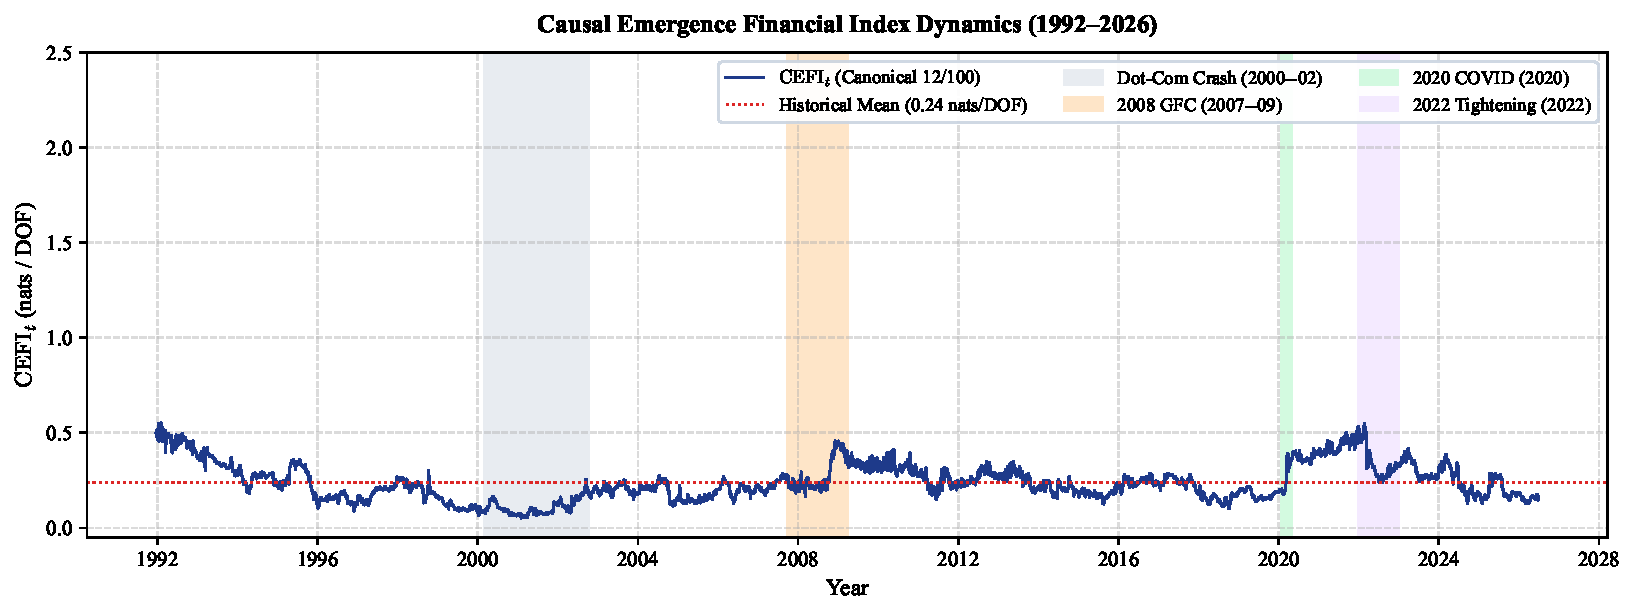
\includegraphics[width=0.95\textwidth]{reports/figures/figure1_cefi_dynamics.pdf}
\caption{Historical dynamics of the Causal Emergence Financial Index ($\mathrm{CEFI}_t$, 1992--2026). Shaded areas indicate historical benchmark stress episodes.}
\label{fig:cefi_dynamics}
\end{figure}

The results in Table \ref{tab:null_models} and Figure \ref{fig:cefi_dynamics} show that:
\begin{enumerate}
    \item In the 2005 calm-market benchmark window, observed $\mathrm{CEFI}_t = 0.2023\ \mathrm{nats/DOF}$ ($q^* = 1$) is statistically consistent with surrogate persistence ($H_0^{\text{static}} p_{\text{emp}} = 0.1160, p_{\text{Holm}} = 0.3480$; $H_0^{\text{diag+contemp}} p_{\text{emp}} = 0.2059, p_{\text{Holm}} = 0.4118$).
    \item During the 2008 GFC peak (November 2008), observed $\mathrm{CEFI}_t = 0.3656\ \mathrm{nats/DOF}$ ($q^* = 1$) approaches the single-test nominal significance boundary against both the static correlation null ($p_{\text{emp}} = 0.0587, z = +1.70, p_{\text{Holm}} = 0.2860$) and the cross-lag network isolation null ($p_{\text{emp}} = 0.0572, z = +1.70, p_{\text{Holm}} = 0.2860$).
    \item During the March 2020 COVID shock, observed $\mathrm{CEFI}_t = 0.3342\ \mathrm{nats/DOF}$ ($q^* = 2$) nominally exceeds the static correlation mode null ($p_{\text{emp}} = 0.0182, z = +2.40, p_{\text{Holm}} = 0.1092$), while remaining statistically consistent with cross-lag isolation ($p_{\text{emp}} = 0.2893, p_{\text{Holm}} = 0.4118$).
\end{enumerate}
Importantly, after Holm-Bonferroni adjustment across the primary hypothesis family ($m=6$), none of the individual tests reject at the 5\% family-wise significance level ($p_{\text{Holm}} \ge 0.1092$). The descriptive excess of observed emergence over the cross-lag network isolation null ($\mathrm{CEFI}_{\text{obs}} - \mathbb{E}[\mathrm{CEFI}_0^{\text{diag+contemp}}]$) is larger at the GFC peak (+0.0778 nats/DOF) than at the 2005 calm benchmark (+0.0370 nats/DOF), although the corresponding primary null comparison does not reject after multiplicity adjustment.

\begin{figure}[htbp]
\centering
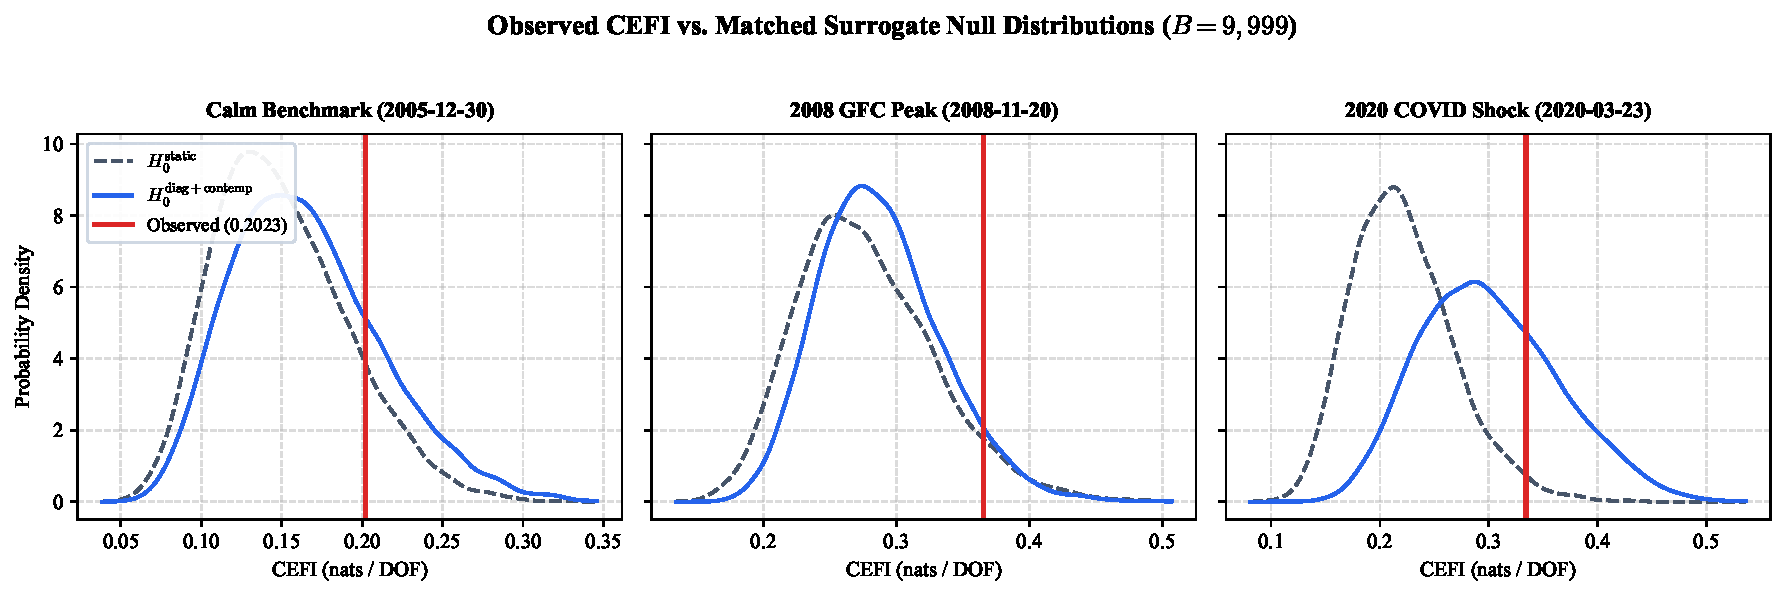
\includegraphics[width=0.95\textwidth]{reports/figures/figure3_null_distributions.pdf}
\caption{Observed $\mathrm{CEFI}_{\text{obs}}$ (red vertical line) compared against matched surrogate null distributions of $H_0^{\text{static}}$ and $H_0^{\text{diag+contemp}}$ across benchmark regimes ($B=9,999$). Empirical $p$-values reported in Table \ref{tab:null_models} are Monte Carlo empirical tail probabilities computed with the $+1$ correction from the surrogate simulations.}
\label{fig:null_dist}
\end{figure}

\subsection{Response Across Historical Episodes: Descriptive Regime Evidence}
To examine whether $\mathrm{CEFI}_t$ behaves differently across historical market stress episodes, we report disaggregated episode-level summary statistics in Table \ref{tab:episode_summary}.

\begin{table}[htbp]
\centering
\caption{Disaggregated Historical Episode Summary Statistics (12 Restarts / 100 Iterations; Units: $\mathrm{nats/DOF}$)}
\label{tab:episode_summary}
\resizebox{\textwidth}{!}{
\begin{tabular}{llccccccc}
\toprule
\textbf{Episode} & \textbf{Stress Class} & \textbf{Obs} & \textbf{Mean } $\mathbf{CEFI}$ & \textbf{Median } $\mathbf{CEFI}$ & \textbf{Modal } $\mathbf{q^*}$ & $\mathbf{P(q^* \le 4)}$ & $\mathbf{P(q^* \le 2)}$ \\
\midrule
Dot-Com Crash (2000--02)  & Valuation Repricing & 327 & 0.1076 & 0.0966 & 2 & 92.7\% & 76.2\% \\
2008 GFC (2007--09)       & Liquidity/Contagion & 189 & 0.2764 & 0.2319 & 1 & 98.9\% & 82.6\% \\
2020 COVID (2020)         & Liquidity/Contagion & 31  & 0.2792 & 0.3172 & 2 & 100.0\% & 100.0\% \\
2022 Tightening (2022)    & Valuation Repricing & 125 & 0.3396 & 0.3166 & 1 & 100.0\%  & 95.9\% \\
\midrule
All Systemic Liquidity    & Pooled Liquidity    & 220 & 0.2768 & 0.2331 & 1 & 99.1\% & 83.7\% \\
All Valuation Repricing   & Pooled Valuation    & 452 & 0.1718 & 0.1248 & 1 & 94.7\%  & 80.8\% \\
\midrule
Full Historical Sample (1992--2026) & Full Baseline & 4,346 & 0.2375 & 0.2222 & 1 & 98.94\% & 87.7\% \\
\bottomrule
\end{tabular}
}
\end{table}

We estimate the descriptive event-study regression specification:
\begin{equation}
\mathrm{CEFI}_t = \alpha + \beta_{\text{Liq}} D_t^{\text{Liquidity}} + \beta_{\text{Val}} D_t^{\text{Valuation}} + u_t
\label{eq:h2_reg_spec}
\end{equation}
where $D_t^{\text{Liquidity}} = 1$ during the 2008 GFC and March 2020 COVID crash ($N=220$), and $D_t^{\text{Valuation}} = 1$ during the 2000 Dot-Com crash and 2022 rate tightening ($N=452$).

\begin{table}[htbp]
\centering
\caption{Descriptive Historical Regime Regressions: Sensitivity Across Extended HAC Lag Bandwidths ($L = 20$ to $L = 250$)}
\label{tab:h2_hac}
\resizebox{\textwidth}{!}{
\begin{tabular}{cccccccc}
\toprule
\textbf{HAC Lag ($L$)} & $\mathbf{\beta_{\text{Liq}}}$ & $\mathbf{t\text{-stat}}$ & $\mathbf{\beta_{\text{Val}}}$ & $\mathbf{t\text{-stat}}$ & $\mathbf{\Delta \beta}$ & \textbf{Wald } $\mathbf{t\text{-stat}}$ & \textbf{Wald } $\mathbf{p\text{-val}}$ \\
\midrule
$L = 20$  & +0.034 & +1.36 & -0.071 & -2.90 & +0.105 & +3.11 & $0.0019$ \\
$L = 40$  & +0.034 & +1.08 & -0.071 & -2.20 & +0.105 & +2.40 & $0.0165$ \\
$L = 60$  & +0.034 & +0.99 & -0.071 & -1.90 & +0.105 & +2.12 & $0.0336$ \\
$L = 120$  & +0.034 & +0.99 & -0.071 & -1.50 & +0.105 & +1.83 & $0.0678$ \\
$L = 250$  & +0.034 & +1.26 & -0.071 & -1.33 & +0.105 & +1.71 & $0.0878$ \\
\bottomrule
\end{tabular}
}
\end{table}

Table \ref{tab:h2_hac} shows that across the benchmark episodes analyzed, $\mathrm{CEFI}_t$ was descriptively higher during liquidity and contagion dislocations ($\beta_{\text{Liq}} = +0.034, t = +1.08$ at $L=40$) than during valuation repricing episodes ($\beta_{\text{Val}} = -0.071, t = -2.20$), yielding an estimated contrast of $\Delta \beta = +0.105$ (Wald $t = +2.40, p = 0.0165$). However, because rolling estimation windows share 498 trading days between adjacent steps, mechanical dependence persists across extended lags. Table \ref{tab:h2_hac} demonstrates that the contrast weakens below conventional significance thresholds for extended bandwidths ($L=120, p=0.0678$; $L=250, p=0.0878$). Furthermore, in leave-one-episode-out sensitivity checks (Supplementary Table 7), omitting the Dot-Com crash reduces the contrast to $\Delta \beta = -0.063$ ($t = -1.36, p = 0.1725$). Consequently, these regressions provide descriptive historical-regime evidence across four specific episodes rather than repeated-sample population inference regarding an invariant crisis taxonomy.

\subsection{Behavior of Causal Effective Dimensionality Across Market Regimes}
Table \ref{tab:episode_summary} and Figure \ref{fig:qstar_dynamics} report the distribution of $q_t^*$.

\begin{figure}[htbp]
\centering
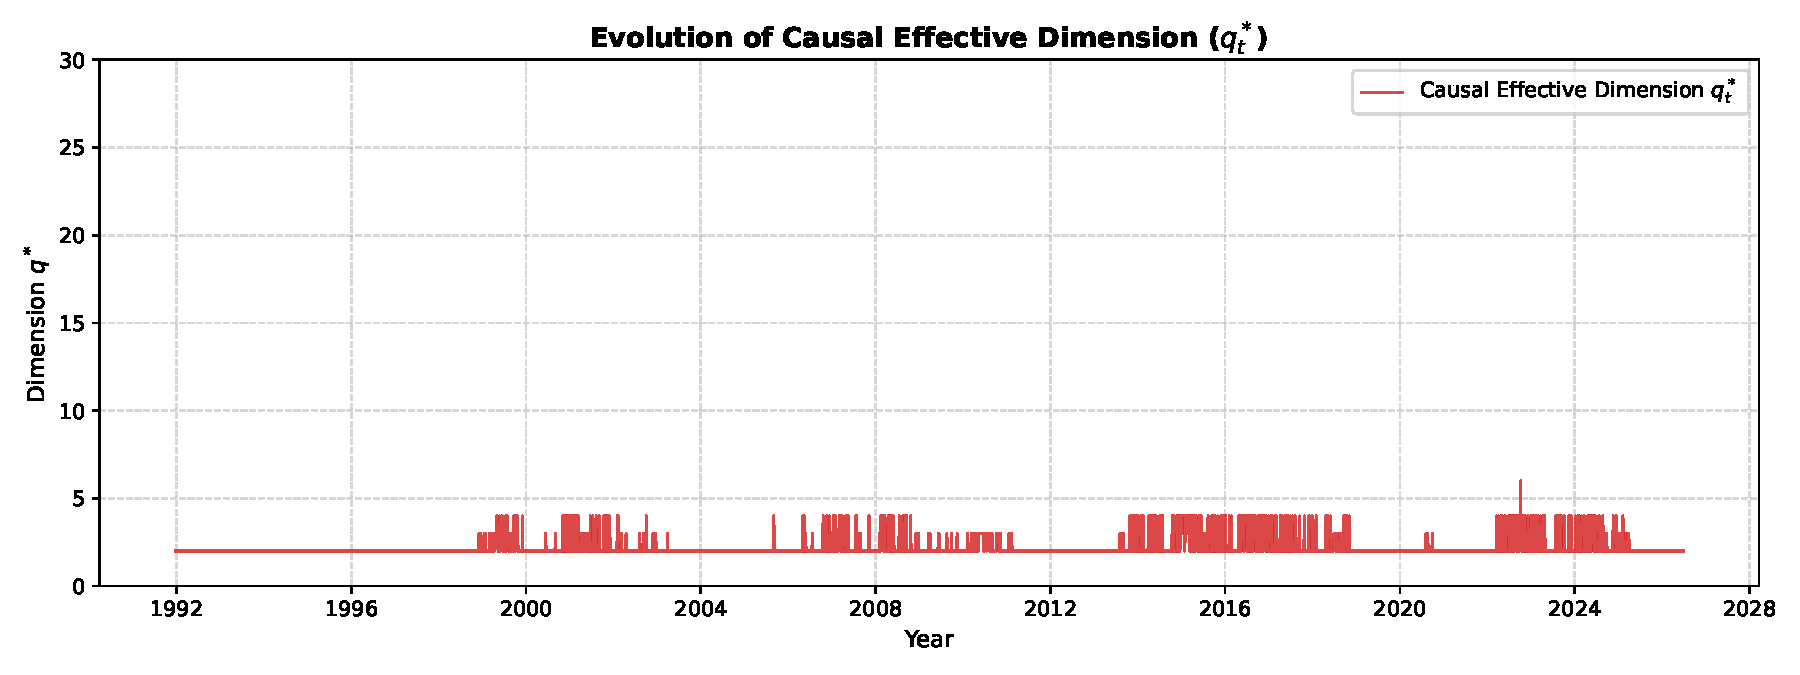
\includegraphics[width=0.95\textwidth]{reports/figures/figure2_qstar_dynamics.pdf}
\caption{Dynamic evolution of the Causal Effective Dimension ($q_t^*$). Shaded areas indicate historical stress episodes.}
\label{fig:qstar_dynamics}
\end{figure}

Across the full 1992--2026 history, 98.94\% of observations exhibit $q^* \le 4$ with modal dimension $q^* = 1$ (accounting for 63.8\% of all windows, and 87.7\% satisfying $q^* \le 2$). Crucially, matched surrogate null models also select modal $q_0^* = 1$ across calm and crisis benchmarks (Table \ref{tab:null_models}), indicating that low dimensional selection is an inherent mathematical property of the per-degree-of-freedom optimization criterion ($\frac{EI_q^*}{q} - \frac{EI_p}{p}$) rather than autonomous empirical evidence of non-null emergent market organization. Moreover, as demonstrated in Section \ref{sec:robustness}, dimensional selection is conditional on the baseline Gaussian intervention scale ($\kappa = 1.0$), with smaller intervention scales shifting modal dimension toward $q^* = 28$. The empirical association between $q^*$ and static Effective Rank across all 4,346 windows is weak (rank correlation $\rho_S = -0.0634$, Pearson $\rho = -0.0781$), showing that $q^*$ is only weakly monotonically associated with static covariance dimensionality.

\subsection{Linear Association with Conventional Systemic Risk Metrics}
To evaluate the relationship between $\mathrm{CEFI}_t$ and standard market metrics, we estimate:
\begin{equation}
\mathrm{CEFI}_t = \alpha + \beta_1 RV_t + \beta_2 \bar{\rho}_t + \beta_3 ER_t + \beta_4 DY_t + u_t
\end{equation}
where $RV_t$ is annualized realized volatility, $\bar{\rho}_t$ is average pairwise correlation, $ER_t = \exp(-\sum_i p_i \ln p_i)$ is effective rank \citep{roy2007effective}, and $DY_t$ is Diebold-Yilmaz total connectedness \citep{diebold2012better} (see Appendix A for formal definitions).

\begin{table}[htbp]
\centering
\caption{Linear Association Between $\mathrm{CEFI}_t$ and Conventional Systemic Risk Benchmarks: Sensitivity Across Extended HAC Lag Bandwidths ($L \in \{40, 120, 250\}$)}
\label{tab:benchmarks_h4}
\resizebox{\textwidth}{!}{
\begin{tabular}{lccccccc}
\toprule
\textbf{Benchmark Proxy} & \textbf{Pairwise Corr} & \textbf{Multivariate } $\mathbf{\beta}$ & \textbf{HAC SE ($L=40$)} & $\mathbf{t\ (L=40)}$ & $\mathbf{t\ (L=120)}$ & $\mathbf{t\ (L=250)}$ & $\mathbf{p\ (L=250)}$ \\
\midrule
Realized Volatility ($RV$)          & +0.425 & +0.3642 & (0.1499) & +2.43 ($p=0.015$) & +1.57 ($p=0.116$) & +1.30 & $0.1937$ \\
Average Correlation ($\bar{\rho}$)  & +0.522 & +0.2876 & (0.2999) & +0.96 ($p=0.338$) & +0.63 ($p=0.529$) & +0.51 & $0.6111$ \\
Effective Rank ($ER$)               & -0.492 & +0.0118 & (0.0121) & +0.98 ($p=0.329$) & +0.62 ($p=0.534$) & +0.50 & $0.6138$ \\
Diebold-Yilmaz Index ($DY$)         & +0.499 & +0.0046 & (0.0048) & +0.96 ($p=0.336$) & +0.64 ($p=0.522$) & +0.54 & $0.5887$ \\
\midrule
\multicolumn{8}{l}{$R^2 = 29.31\% \qquad \text{Unexplained Linear Variance} = 70.69\% \qquad N = 4,346$} \\
\bottomrule
\end{tabular}
}
\end{table}

Standard systemic risk proxies account for 29.31\% of the in-sample linear variation in $\mathrm{CEFI}_t$, while 70.69\% remains unexplained by this linear combination, indicating that a substantial share of $\mathrm{CEFI}_t$ variation is not linearly spanned by this set of conventional proxies. However, Table \ref{tab:benchmarks_h4} reveals that when accounting for mechanical rolling window overlap via extended HAC lag bandwidths ($L=120$ and $L=250$), even realized volatility ceases to be statistically significant ($t=1.57, p=0.1159$ and $t=1.30, p=0.1937$), while correlation, effective rank, and connectedness remain statistically insignificant across all bandwidths ($p \ge 0.3288$). Collinearity diagnostics yield $\text{VIF}(RV) = 3.20$, $\text{VIF}(\bar{\rho}) = 27.30$, $\text{VIF}(ER) = 13.77$, and $\text{VIF}(DY) = 15.11$ (condition number $= 11.80$). Residualized $\mathrm{CEFI}_t = \mathrm{CEFI}_t - \hat{\mathbb{E}}[\mathrm{CEFI}_t \mid RV, \bar{\rho}, ER, DY]$ exhibits episode-specific variation. Mean residualized $\mathrm{CEFI}_t$ is close to zero during the GFC and COVID episode windows ($-0.0025$ and $+0.0017$), whereas larger episode-average residuals occur during the Dot-Com and 2022 repricing episodes ($-0.0496$ and $+0.0941$).

\section{Robustness and Cross-Method Theoretical Benchmarking}
\label{sec:robustness}

\subsection{Cross-Method Benchmarking Against Published Literature}
Table \ref{tab:cross_framework} and Figure \ref{fig:cross_framework} report cross-method concordance across 870 historical rolling windows.

\begin{table}[htbp]
\centering
\caption{Cross-Method Benchmarking Against Published Literature (1992--2026, 870 Rolling Slices)}
\label{tab:cross_framework}
\resizebox{\textwidth}{!}{
\begin{tabular}{lcccc}
\toprule
\textbf{Theoretical Benchmark} & \textbf{Pearson } $\mathbf{\rho}$ & \textbf{Spearman } $\mathbf{\rho_S}$ & \textbf{Exact } $\mathbf{q^*}$ \textbf{Match} & $\mathbf{q^*}$ \textbf{Match (}$\pm 1$\textbf{)} \\
\midrule
Liu et al. (2024) Uniform $\Delta \mathcal{J}$ & 0.445 & 0.356 & 9.0\% & 10.7\% \\
Liu et al. (2025) SVD Emergence           & 0.819 & 0.821 & 63.2\% & \textbf{87.7\%} \\
\bottomrule
\end{tabular}
}
\end{table}

\begin{figure}[htbp]
\centering
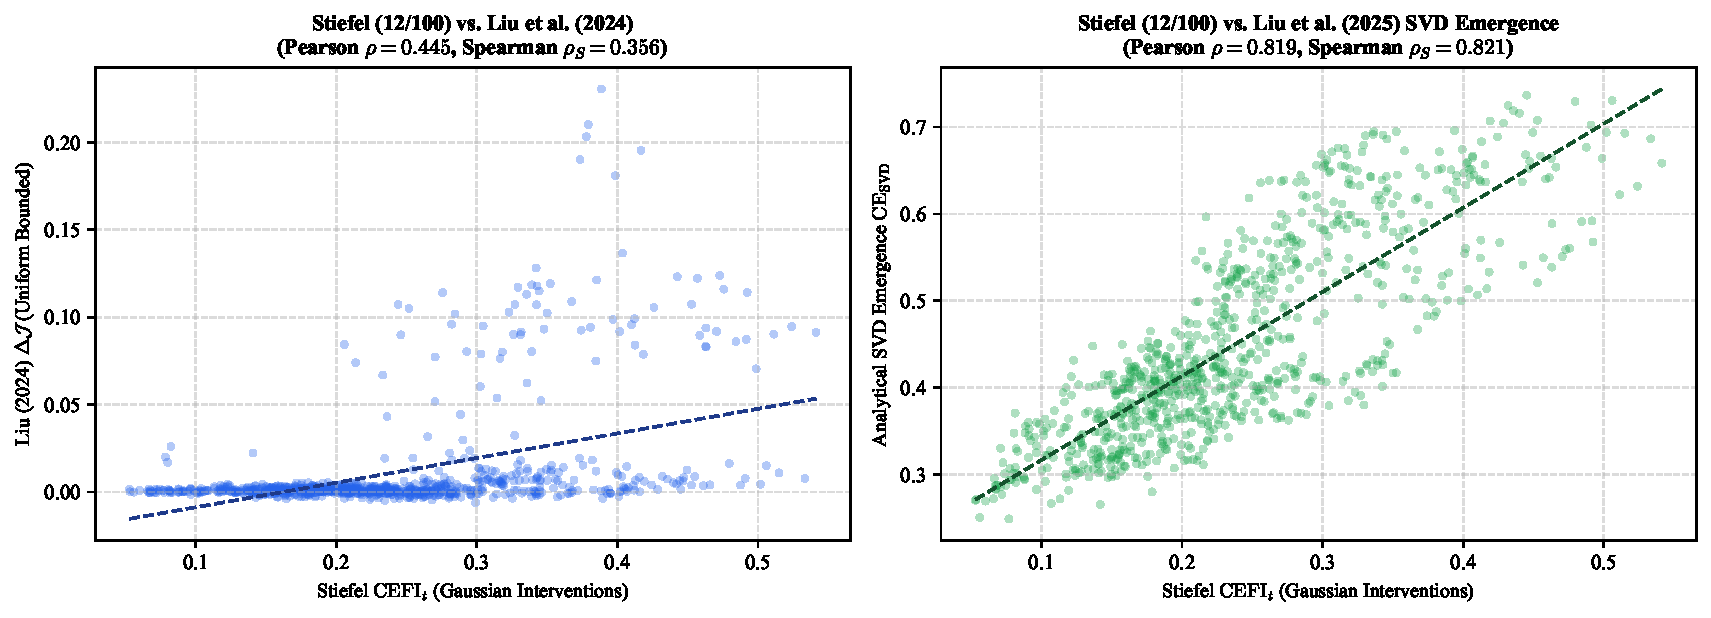
\includegraphics[width=0.90\textwidth]{reports/figures/figure4_theoretical_benchmarking.pdf}
\caption{Cross-method benchmarking across 870 historical slices: (a) $\mathrm{CEFI}_t$ vs. exact $\Delta \mathcal{J}$ of \citet{liu2024exact}; (b) $\mathrm{CEFI}_t$ vs. analytical SVD emergence of \citet{liu2025singular}.}
\label{fig:cross_framework}
\end{figure}

The Stiefel manifold index is positively associated with the analytical Gaussian SVD emergence of \citet{liu2025singular} (Pearson $\rho = 0.819$, Spearman $\rho_S = 0.821$) with 87.7\% dimensional agreement within $\pm 1$ dimension (63.2\% exact dimensional match) across all 870 rolling slices. This concordance indicates that the numerical Stiefel optimizer aligns closely with the analytical Gaussian SVD emergence benchmark under equivalent Gaussian intervention assumptions; it does not, however, constitute external or independent validation of economic risk content. In contrast, the formulation of \citet{liu2024exact} evaluates bounded uniform interventions, yielding moderate empirical correlation ($\rho = 0.445, \rho_S = 0.356$) and lower dimensional agreement (9.0\% exact match), consistent with sensitivity of continuous causal-emergence estimates to the intervention geometry.

\subsection{Cross-Partition and Industry-Granularity Sensitivity (FF49 Replication)}
Evaluating the framework across all $q \in \{1, \dots, 48\}$ on the 49 Industry Portfolios ($p=49$) under the 12/100 budget yields a mean $\mathrm{CEFI}$ of 0.3592\ $\mathrm{nats/DOF}$ (median 0.3483) and a modal dimension of $q^* = 1$, with 97.13\% of historical windows exhibiting $q^* \le 4$. These exploratory cross-partition results confirm persistent low-dimensional optimizer selection under finer industrial granularity within the same underlying U.S. equity market.

\subsection{Sensitivity to Scale Parameter \texorpdfstring{$\kappa$}{kappa} and Window Size \texorpdfstring{$W$}{W}}
Varying the intervention strength across $\kappa \in \{0.25, 0.50, 1.00, 2.00, 4.00\}$ preserves moderate-to-high rank concordance with the baseline ($\rho_S \in [0.688, 1.000]$, Table \ref{tab:kappa_sensitivity}), with modal $q^* = 1$ for $\kappa \ge 1.00$. For very small intervention scales ($\kappa = 0.25$), the modal dimension shifts to $q^* = 28$, demonstrating that effective-dimension selection is conditional on the baseline intervention scale before stabilizing at $q^* \in \{1, 3\}$ for $\kappa \ge 0.50$. Increasing estimation windows to $W = 750$ and $W = 1000$ trading days yields rank correlations of $\rho_S = 0.819$ and $\rho_S = 0.690$ (Table \ref{tab:window_sensitivity}), with optimal phase lags of $\ell = -10$ and $\ell = -140$ trading days, reflecting mechanical rolling window smoothing.

\section{Discussion}
\label{sec:discussion}

\subsection{Economic Interpretation of Financial Causal Emergence}
A positive $\mathrm{CEFI}_t$ indicates that an optimal macroscopic coarse-graining of the financial system possesses a higher causal transition density than the disaggregated micro-level assets. In economic terms, when individual industries experience elevated idiosyncratic noise, a properly oriented lower-dimensional projection can eliminate mutually cancelling noise components while concentrating collective intertemporal momentum.

\subsection{Disentangling Contemporaneous Co-Movement from Lagged Dynamical Structure}
Our four-tier null hierarchy clarifies the distinction between static correlation and dynamic causal organization. In the 2005 calm benchmark, observed emergence ($\mathrm{CEFI}_{\text{obs}} = 0.2023\ \mathrm{nats/DOF}$) is consistent with surrogate persistence ($p_{\text{Holm}} \ge 0.3480$), with a modest excess over the cross-lag network isolation null ($+0.0370\ \mathrm{nats/DOF}$). In contrast, during major systemic stress episodes, descriptive emergence increases: during the 2008 GFC peak, the descriptive excess over the cross-lag network isolation null is $+0.0778\ \mathrm{nats/DOF}$ ($p_{\text{emp}} = 0.0572, p_{\text{Holm}} = 0.2860$), while during the March 2020 COVID shock, observed emergence nominally exceeds static correlation modes ($\mathrm{CEFI}_{\text{obs}} = 0.3342\ \mathrm{nats/DOF}$ vs. $\mathbb{E}[\mathrm{CEFI}_0] = 0.2213$, $z = +2.40, p_{\text{emp}} = 0.0182, p_{\text{Holm}} = 0.1092$), while remaining consistent with cross-lag isolation ($p_{\text{emp}} = 0.2893$). Crucially, because no primary test survives Holm adjustment, these regime differences provide descriptive historical-regime evidence rather than definitive inferential proof of state-dependent cross-lag intensifying.

\subsection{Inter-Crisis Episodes (2011--2013 Debt Ceiling and Sovereign Debt)}
As shown in Figure \ref{fig:cefi_dynamics}, $\mathrm{CEFI}_t$ also displays secondary peaks during the 2011 U.S. sovereign debt downgrade and the European sovereign debt crisis. These peaks coincide with known macro-financial stress events. However, because matched-null inference was not conducted for every historical window, their interpretation as dynamic cross-sectoral organization remains descriptive.

\subsection{Complementarity with Macroprudential Indicators}
These results suggest that causal emergence may provide a complementary information-theoretic lens for monitoring changes in systemic market organization, capturing shifts in collective transition structure that supplement traditional static correlation and volatility indices.

\section{Limitations}
\label{sec:limitations}

Several methodological limitations should be noted:
\begin{enumerate}
    \item \textbf{Optimizer Search Budget Sensitivity}: While the production 12-restart/100-iteration configuration exhibits high concordance (Pearson $\rho = 0.9732$, Spearman $\rho_S = 0.9377$, 92.0\% exact $q^*$ match, 100.0\% match within $\pm 1$, median gap 1.82\%) relative to the 25-restart/150-iteration high-budget reference configuration, exact objective values remain subject to numerical search budgets on non-convex manifolds.
    \item \textbf{Linear Gaussian Transition Dynamics}: Micro-dynamics are modeled through a linear VAR(1) with Gaussian innovations. Non-linear spillover dynamics, volatility clustering, and heavy-tailed co-jumps are not explicitly parameterized in the transition operator.
    \item \textbf{Reduced-Form Representation}: The transition matrix $\mathbf{A}$ is estimated in reduced form. Interventions represent counterfactual Gaussian perturbations under the fitted dynamical model and should not be interpreted as structural policy shocks.
    \item \textbf{Generated-Statistic Uncertainty}: $\mathrm{CEFI}_t$ is a generated statistic obtained from first-stage parameter estimates ($\hat{\mathbf{A}}, \boldsymbol{\Sigma}_\varepsilon, \mathbf{W}, q^*$). Downstream HAC regressions do not fully propagate first-stage estimation uncertainty.
    \item \textbf{Aggregation Level}: The empirical analysis relies on industry portfolios rather than individual financial institutions, reflecting cross-sectoral market organization rather than interbank counterparty networks.
    \item \textbf{Sample Size of Historical Crises}: The number of major systemic dislocations in modern market history is inherently limited. Event-study inference should be interpreted as within-sample regime evidence across historical episodes rather than asymptotic identification of crisis taxonomies.
    \item \textbf{Intervention Family Dependence}: Although CEFI rankings remain moderately to strongly concordant across the evaluated intervention scales, effective-dimension selection becomes sensitive at small intervention amplitudes, particularly at $\kappa = 0.25$, and $\mathrm{CEFI}_t$ remains conditional on the chosen family of isotropic Gaussian interventions.
    \item \textbf{Absence of Early-Warning Validation}: The empirical design evaluates concurrent market organization during stress regimes; no early-warning or predictive lead-time capability is claimed or validated.
\end{enumerate}

\section{Conclusion}
\label{sec:conclusion}

This paper has developed and evaluated continuous-state Causal Emergence as an empirical measure of dynamic cross-sectoral market organization during systemic stress in U.S. equity industry portfolios. By formulating scale-invariant Effective Information on Stiefel manifolds and benchmarking against a hierarchy of matched surrogate null models ($B=9,999$ for primary nulls and $B=999$ for auxiliary nulls), we document that cross-industry return dynamics exhibit a persistently low causal effective dimension ($q^* \le 2$ in 87.7\% of rolling windows, $q^* \le 4$ in 98.94\%, modal $q^* = 1$ accounting for 63.8\% of all windows) under baseline Gaussian interventions ($\kappa = 1.0$). Because matched surrogate null models without cross-lag couplings also select modal $q_0^* = 1$, low-dimensional selection is also favored by the per-degree-of-freedom criterion under matched surrogate models, and thus is not, by itself, evidence of non-null emergent structure. Across historical episodes, while emergence is statistically consistent with surrogate persistence in the 2005 calm-market benchmark ($p_{\text{Holm}} \ge 0.3480$), the GFC and COVID benchmark windows exhibit higher observed emergence than the calm benchmark: during the 2008 GFC peak, the descriptive excess over cross-lag network isolation is larger than in the calm baseline (+0.0778 vs. +0.0370 nats/DOF, $p_{\text{emp}} = 0.0572, p_{\text{Holm}} = 0.2860$), while during the March 2020 COVID shock, observed emergence nominally exceeds static correlation modes ($p_{\text{emp}} = 0.0182, z = +2.40, p_{\text{Holm}} = 0.1092$) while remaining consistent with cross-lag isolation ($p_{\text{emp}} = 0.2893$). Continuous causal emergence under Gaussian interventions exhibits strong agreement with analytical SVD emergence ($\rho = 0.819, \rho_S = 0.821$), providing a descriptive information-theoretic framework for monitoring macroscopic market organization during financial distress.

\appendix

\section{Benchmark Construction and Definitions}
\label{app:benchmarks}
Conventional systemic risk proxies are constructed over each rolling window $X_{t-W+1:t}$ as follows:
\begin{enumerate}
    \item \textbf{Realized Volatility ($RV_t$)}: Annualized standard deviation of the equal-weighted portfolio return series, $RV_t = \sqrt{252} \cdot \operatorname{std}(\bar{x}_t)$.
    \item \textbf{Average Correlation ($\bar{\rho}_t$)}: Mean off-diagonal element of the $p \times p$ sample correlation matrix $\mathbf{R}_t$: $\bar{\rho}_t = \frac{2}{p(p-1)} \sum_{i < j} R_{ij,t}$.
    \item \textbf{Effective Rank ($ER_t$)}: Spectral entropy exponentiation of normalized covariance eigenvalues \citep{roy2007effective}:
    \begin{equation}
    ER_t = \exp\left( -\sum_{i=1}^p p_i \ln p_i \right), \qquad p_i = \frac{\lambda_i(\boldsymbol{\Sigma}_{x,t})}{\sum_{j=1}^p \lambda_j(\boldsymbol{\Sigma}_{x,t})}
    \end{equation}
    \item \textbf{Diebold-Yilmaz Connectedness Index ($DY_t$)}: Total volatility spillover index derived from generalized forecast error variance decompositions of a VAR(1) with forecast horizon $H = 10$ days \citep{diebold2012better}.
\end{enumerate}

\section{Optimization Budget Calibration and Multi-Start Stability}
\label{app:optimizer_calibration}

To evaluate numerical stability and search-budget sensitivity on the compact Stiefel manifold $\mathcal{V}_q(\mathbb{R}^p)$, we evaluate the trade-off between optimization accuracy and computational tractability across candidate configurations $(R, K)$, where $R$ denotes the number of deterministic orthogonal multistarts and $K$ the maximum Riemannian gradient ascent iterations. Evaluations are benchmarked against a high-budget reference configuration of $(R_{\mathrm{ref}}=25, K_{\mathrm{ref}}=150)$ across representative market regimes.

\begin{table}[htbp]
\centering
\caption{Optimization Budget Calibration against High-Budget Reference Configuration ($R=25, K=150$).}
\label{tab:optimizer_calibration}
\resizebox{\textwidth}{!}{
\begin{tabular}{lccccccc}
\toprule
\textbf{Configuration } $(R, K)$ & \textbf{Cost Multiplier} & \textbf{Median Gap (\%)} & \textbf{Q95 Gap (\%)} & \textbf{Pearson } $\mathbf{\rho}$ & $\mathbf{q^*}$ \textbf{Exact Match (\%)} & $\mathbf{q^* \pm 1}$ \textbf{Match (\%)} \\
\midrule
$(R=4, K=35)$ & $1.00\times$ & 25.08\% & 40.74\% & 0.8452 & 52.0\% & 88.0\% \\
$(R=8, K=75)$ & $2.90\times$ & 5.31\% & 16.84\% & 0.9533 & 72.0\% & 84.0\% \\
$\mathbf{(R=12, K=100)}$ \textbf{[Production]} & $\mathbf{5.90\times}$ & \textbf{1.82\%} & \textbf{11.70\%} & \textbf{0.9732} & \textbf{92.0\%} & \textbf{100.0\%} \\
$(R=16, K=100)$ & $7.84\times$ & 1.20\% & 8.39\% & 0.9756 & 88.0\% & 92.0\% \\
$(R=25, K=150)$ [Reference] & $18.02\times$ & 0.00\% & 0.00\% & 1.0000 & 100.0\% & 100.0\% \\
\bottomrule
\end{tabular}
}
\begin{minipage}{\textwidth}
\vspace{4pt}
\scriptsize \emph{Notes:} Evaluated across 25 representative historical estimation windows on the dimension-selection objective $J(q^*) = \frac{EI_{q^*}}{q^*} - \frac{EI_p}{p}$. The production specification $(R=12, K=100)$ matches the dimension selected by the high-budget reference in 92.0\% of test windows and within $\pm 1$ dimension in 100.0\% of cases (Pearson $\rho = 0.9732$, Spearman $\rho_S = 0.9377$), with a median objective gap of 1.82\%, while strictly applying identical computational budgets to observed windows and surrogate null realizations to avoid differential optimization-budget bias.
\end{minipage}
\end{table}

\section{Supplementary Robustness Tables}
\label{app:robustness_tables}

\begin{table}[htbp]
\centering
\caption{Sensitivity to the Intervention Scale Parameter $\kappa_{do}$.}
\label{tab:kappa_sensitivity}
\resizebox{\textwidth}{!}{
\begin{tabular}{lccccc}
\toprule
\textbf{Intervention Scale } $\mathbf{\kappa_{do}}$ & \textbf{Mean CEFI} & \textbf{Spearman } $\mathbf{\rho}$ \textbf{vs. Baseline} & \textbf{Modal } $\mathbf{q^*}$ & $\mathbf{\beta_{\mathrm{Liq}}}$ & $\mathbf{t}$\textbf{-stat (HAC)} \\
\midrule
$\kappa = 0.25$ & 0.0005 & 0.6879 & 28 & 0.0015 & 1.27 \\
$\kappa = 0.50$ & 0.0316 & 0.8386 & 3  & 0.0205 & 1.04 \\
$\mathbf{\kappa = 1.00}$ \textbf{[Baseline]} & \textbf{0.2375} & \textbf{1.0000} & \textbf{1} & \textbf{0.0336} & \textbf{1.08} \\
$\kappa = 2.00$ & 0.5146 & 0.8935 & 1  & 0.0231 & 0.68 \\
$\kappa = 4.00$ & 0.7729 & 0.7887 & 1  & -0.0038 & -0.12 \\
\bottomrule
\end{tabular}
}
\end{table}

\begin{table}[htbp]
\centering
\caption{Sensitivity to Estimation Window Length $W$.}
\label{tab:window_sensitivity}
\resizebox{\textwidth}{!}{
\begin{tabular}{lcccc}
\toprule
\textbf{Window Length} & \textbf{Mean CEFI} & \textbf{Spearman } $\mathbf{\rho}$ \textbf{vs. Baseline} & \textbf{Phase Lag (Trading Days)} & \textbf{Lagged Correlation} \\
\midrule
$W = 500$ (Baseline, 2 years) & 0.2375 & 1.0000 & 0 & 1.0000 \\
$W = 750$ (3 years)           & 0.1676 & 0.8186 & -10 & 0.7933 \\
$W = 1000$ (4 years)          & 0.1250 & 0.6896 & -140 & 0.6798 \\
\bottomrule
\end{tabular}
}
\end{table}

\begin{table}[htbp]
\centering
\caption{Observational Closure Diagnostics at Optimal Macro-Dimension $q^*$.}
\label{tab:closure_diagnostics}
\resizebox{\textwidth}{!}{
\begin{tabular}{lcccc}
\toprule
\textbf{Market Episode} & \textbf{Benchmark Date} & \textbf{Optimal } $\mathbf{q^*}$ & \textbf{Closure Ratio } $\mathbf{r_{\mathrm{closure}}}$ & \textbf{Observational Status} \\
\midrule
2005 Calm Benchmark   & 2005-12-30 & 1 & 0.3915 & Structurally Open \\
2008 GFC Peak         & 2008-11-20 & 1 & 0.4350 & Structurally Open \\
2020 COVID Crash      & 2020-03-23 & 2 & 0.4826 & Structurally Open \\
2000 Dot-Com Crash    & 2001-03-20 & 6 & 0.4560 & Structurally Open \\
2022 Rate Tightening  & 2022-06-15 & 1 & 0.4637 & Structurally Open \\
\bottomrule
\end{tabular}
}
\begin{minipage}{\textwidth}
\vspace{4pt}
\scriptsize \emph{Notes:} The non-zero closure ratios ($r_{\mathrm{closure}} \in [0.39, 0.48] > 0$) indicate that the optimized macro representations are not observationally closed; $\mathbf{W}\mathbf{A}\mathbf{W}^\top$ is therefore interpreted throughout as the transition operator of the constructed interventional macro channel rather than an autonomous observational system.
\end{minipage}
\end{table}

\section*{Declaration of Competing Interests}
The author declares that they have no known competing financial interests or personal relationships that could have appeared to influence the work reported in this paper.

\section*{Data and Code Availability}
All datasets used in this study (Kenneth French 30 and 49 Industry Portfolios) are publicly available from the Kenneth French Data Library (\url{https://mba.tuck.dartmouth.edu/pages/faculty/ken.french/data_library.html}). Complete replication code, numerical optimization routines, surrogate null generators, and pipeline automation scripts are maintained in an anonymized replication repository and will be made publicly available with a permanent open-access DOI upon acceptance and publication, accompanied by reproduction scripts and frozen random seeds for complete computational provenance.

\section*{Declaration of Generative AI and AI-Assisted Technologies in the Writing Process}
During the preparation of this work, the author used OpenAI GPT in order to edit language, improve readability, and adapt the writing of the manuscript. After using this tool, the author reviewed and edited the content as needed and takes full responsibility for the content of the publication.

\bibliographystyle{elsarticle-harv}
\begin{thebibliography}{28}
\bibitem[Absil et~al., 2008]{absil2008optimization}
Absil, P.-A., Mahony, R., Sepulchre, R., 2008.
\newblock Optimization Algorithms on Matrix Manifolds.
\newblock Princeton University Press, Princeton, NJ. \url{https://doi.org/10.1515/9781400830244}

\bibitem[Acharya et~al., 2017]{acharya2017measuring}
Acharya, V. V., Pedersen, L. H., Philippon, T., Richardson, M., 2017.
\newblock Measuring Systemic Risk.
\newblock \emph{Review of Financial Studies} 30(1), 2--47. \url{https://doi.org/10.1093/rfs/hhw088}

\bibitem[Adrian and Brunnermeier, 2016]{adrian2016covar}
Adrian, T., Brunnermeier, M. K., 2016.
\newblock CoVaR.
\newblock \emph{American Economic Review} 106(7), 1705--1741. \url{https://doi.org/10.1257/aer.20120555}

\bibitem[Ahelegbey et~al., 2022]{ahelegbey2022network}
Ahelegbey, D. F., Cerchiello, P., Scaramozzino, R., 2022.
\newblock Network based evidence of the financial impact of Covid-19 pandemic.
\newblock \emph{International Review of Financial Analysis} 81, 102101. \url{https://doi.org/10.1016/j.irfa.2022.102101}

\bibitem[Ardakani, 2024]{ardakani2024transfer}
Ardakani, O.~M., 2024.
\newblock Portfolio optimization with transfer entropy constraints.
\newblock \emph{International Review of Financial Analysis} 96, 103644. \url{https://doi.org/10.1016/j.irfa.2024.103644}

\bibitem[Barun{\'i}k and K{\v{r}}ehl{\'i}k, 2018]{barunik2018measuring}
Barun{\'i}k, J., K{\v{r}}ehl{\'i}k, T., 2018.
\newblock Measuring the frequency dynamics of financial connectedness and systemic risk.
\newblock \emph{Journal of Financial Econometrics} 16(2), 271--296. \url{https://doi.org/10.1093/jjfinec/nby001}

\bibitem[Bekiros et~al., 2017]{bekiros2017information}
Bekiros, S., Nguyen, D. K., Uddin, G. S., Sjo, B., 2017.
\newblock Information diffusion, cluster formation and entropy-based network dynamics in equity and commodity markets.
\newblock \emph{European Journal of Operational Research} 256(3), 945--961. \url{https://doi.org/10.1016/j.ejor.2016.06.052}

\bibitem[Billio et~al., 2012]{billio2012econometric}
Billio, M., Getmansky, M., Lo, A. W., Pelizzon, L., 2012.
\newblock Econometric measures of connectedness and systemic risk in the finance and insurance sectors.
\newblock \emph{Journal of Financial Economics} 104(3), 535--559. \url{https://doi.org/10.1016/j.jfineco.2011.12.010}

\bibitem[Bouri et~al., 2021]{bouri2021return}
Bouri, E., Cepni, O., Gabauer, D., Gupta, R., 2021.
\newblock Return connectedness across asset classes around the COVID-19 outbreak.
\newblock \emph{International Review of Financial Analysis} 73, 101646. \url{https://doi.org/10.1016/j.irfa.2020.101646}

\bibitem[Brownlees and Engle, 2017]{brownlees2017srisk}
Brownlees, C., Engle, R. F., 2017.
\newblock SRISK: A conditional capital shortfall measure of systemic risk.
\newblock \emph{Review of Financial Studies} 30(1), 48--79. \url{https://doi.org/10.1093/rfs/hhw060}

\bibitem[Demirer et~al., 2018]{demirer2018estimating}
Demirer, M., Diebold, F.~X., Liu, L., Yilmaz, K., 2018.
\newblock Estimating global bank network connectedness.
\newblock \emph{Journal of Applied Econometrics} 33(1), 1--15. \url{https://doi.org/10.1002/jae.2585}

\bibitem[Diebold and Yilmaz, 2012]{diebold2012better}
Diebold, F. X., Yilmaz, K., 2012.
\newblock Better to give than to receive: Predictive directional measurement of volatility spillovers.
\newblock \emph{International Journal of Forecasting} 28(1), 57--66. \url{https://doi.org/10.1016/j.ijforecast.2011.02.006}

\bibitem[Diebold and Yilmaz, 2014]{diebold2014network}
Diebold, F. X., Yilmaz, K., 2014.
\newblock On the network topology of variance decompositions: Measuring the connectedness of financial firms.
\newblock \emph{Journal of Econometrics} 182(1), 119--134. \url{https://doi.org/10.1016/j.jeconom.2014.04.012}

\bibitem[Dimpfl and Peter, 2013]{dimpfl2013using}
Dimpfl, T., Peter, F. J., 2013.
\newblock Using transfer entropy to measure dynamic information flows between markets.
\newblock \emph{Journal of International Financial Markets, Institutions and Money} 27, 273--294. \url{https://doi.org/10.1016/j.intfin.2013.09.003}

\bibitem[Edelman et~al., 1998]{edelman1998geometry}
Edelman, A., Arias, T. A., Smith, S. T., 1998.
\newblock The geometry of algorithms with orthogonality constraints.
\newblock \emph{SIAM Journal on Matrix Analysis and Applications} 20(2), 303--353. \url{https://doi.org/10.1137/S0895479895290954}

\bibitem[Hoel, 2017]{hoel2017when}
Hoel, E. P., 2017.
\newblock When the map is better than the territory.
\newblock \emph{Entropy} 19(5), 188. \url{https://doi.org/10.3390/e19050188}

\bibitem[Hoel et~al., 2013]{hoel2013quantifying}
Hoel, E. P., Albantakis, L., Tononi, G., 2013.
\newblock Quantifying causal emergence shows that macro can beat micro.
\newblock \emph{Proceedings of the National Academy of Sciences} 110(49), 19790--19795. \url{https://doi.org/10.1073/pnas.1314922110}

\bibitem[Klein and Hoel, 2020]{klein2020emergence}
Klein, B., Hoel, E., 2020.
\newblock The emergence of informative higher scales in complex networks.
\newblock \emph{Complexity} 2020, 8932526. \url{https://doi.org/10.1155/2020/8932526}

\bibitem[Kritzman et~al., 2011]{kritzman2011principal}
Kritzman, M., Li, Y., Page, S., Rigobon, R., 2011.
\newblock Principal components as a measure of systemic risk.
\newblock \emph{Journal of Portfolio Management} 37(4), 112--126. \url{https://doi.org/10.3905/jpm.2011.37.4.112}

\bibitem[Ledoit and Wolf, 2004]{ledoit2004well}
Ledoit, O., Wolf, M., 2004.
\newblock A well-conditioned estimator for large-dimensional covariance matrices.
\newblock \emph{Journal of Multivariate Analysis} 88(2), 365--411. \url{https://doi.org/10.1016/S0047-259X(03)00096-4}

\bibitem[Liu et~al., 2024]{liu2024exact}
Liu, K., Yuan, B., Zhang, J., 2024.
\newblock An exact theory of causal emergence for linear stochastic iteration systems.
\newblock \emph{Entropy} 26(8), 618. \url{https://doi.org/10.3390/e26080618}

\bibitem[Liu et~al., 2025]{liu2025singular}
Liu, K., Pan, L., Wang, Z., Yang, M., Yuan, B., Zhang, J., 2025.
\newblock Singular-value-decomposition-based causal emergence for Gaussian iterative systems.
\newblock \emph{Physical Review E} 112(5), 054225. \url{https://doi.org/10.1103/mfct-sxn5}

\bibitem[Mensi et~al., 2021]{mensi2021spillovers}
Mensi, W., Hernandez, J. A., Yoon, S.-M., Vo, X. V., Kang, S. H., 2021.
\newblock Spillovers and connectedness between major precious metals and major currency markets: The role of frequency factor.
\newblock \emph{International Review of Financial Analysis} 74, 101672. \url{https://doi.org/10.1016/j.irfa.2021.101672}

\bibitem[Newey and West, 1987]{newey1987hypothesis}
Newey, W. K., West, K. D., 1987.
\newblock A simple, positive semi-definite, heteroskedasticity and autocorrelation consistent covariance matrix.
\newblock \emph{Econometrica} 55(3), 703--708. \url{https://doi.org/10.2307/1913610}

\bibitem[Politis and Romano, 1994]{politis1994stationary}
Politis, D. N., Romano, J. P., 1994.
\newblock The stationary bootstrap.
\newblock \emph{Journal of the American Statistical Association} 89(428), 1303--1313. \url{https://doi.org/10.1080/01621459.1994.10476870}

\bibitem[Rosas et~al., 2020]{rosas2020reconciling}
Rosas, F. E., Mediano, P. A., Jensen, H. J., Seth, A. K., Barrett, A. B., Carhart-Harris, R. L., Bor, D., 2020.
\newblock Reconciling emergences: An information-theoretic approach to identify causal emergence in multivariate data.
\newblock \emph{PLoS Computational Biology} 16(12), e1008579. \url{https://doi.org/10.1371/journal.pcbi.1008579}

\bibitem[Roy and Vetterli, 2007]{roy2007effective}
Roy, O., Vetterli, M., 2007.
\newblock The effective rank: A measure of effective dimensionality.
\newblock 15th European Signal Processing Conference (EUSIPCO 2007), 606--610.

\bibitem[Schreiber, 2000]{schreiber2000measuring}
Schreiber, T., 2000.
\newblock Measuring information transfer.
\newblock \emph{Physical Review Letters} 85(2), 461--464. \url{https://doi.org/10.1103/PhysRevLett.85.461}

\bibitem[Yang et~al., 2025]{yang2025finding}
Yang, M., Wang, Z., Liu, K., Rong, Y., Yuan, B., Zhang, J., 2025.
\newblock Finding emergence in data by maximizing effective information.
\newblock \emph{National Science Review} 12(1), nwae279. \url{https://doi.org/10.1093/nsr/nwae279}

\bibitem[Yang and Hamori, 2023]{yang2023modeling}
Yang, L., Hamori, S., 2023.
\newblock Modeling the global sovereign credit network under climate change.
\newblock \emph{International Review of Financial Analysis} 87, 102618. \url{https://doi.org/10.1016/j.irfa.2023.102618}

\bibitem[Yao and Li, 2025]{yao2025interindustry}
Yao, C.-Z., Li, Y.-L., 2025.
\newblock Structural evolution of industry association networks in Chinese stock market under major event shocks: A comparative analysis of two crises based on partial Granger causal networks.
\newblock \emph{International Review of Financial Analysis} 107, 104572. \url{https://doi.org/10.1016/j.irfa.2025.104572}

\bibitem[Yousaf et~al., 2022]{yousaf2022linkages}
Yousaf, I., Nekhili, R., Gubareva, M., 2022.
\newblock Linkages between DeFi assets and conventional currencies: Evidence from the COVID-19 pandemic.
\newblock \emph{International Review of Financial Analysis} 81, 102082. \url{https://doi.org/10.1016/j.irfa.2022.102082}
\end{thebibliography}

\end{document}
